%Created on: May 8, 2014        Edited by: Wesley Kyle
%Edited on:	May 16, 2016	Edited by: P. Gimby - fixed page numbering error.
%Edited on: May 20, 2016        Edited by: P. Gimby - replaced preamble with input from external file - added tages for easy removal of prelab questions
%Edited on: Aug 23, 2016	Edited by: W.Kyle - Corrected typos and formating issues
%Edited on: Aug 23, 2017	Edited by: Ania Harlick
% Beginning code for all standard physics latex documents

%Created on: May 8, 2014    Edited by: Wesley Kyle
%Edited on:	May 12, 2016	Edited by: P. Gimby - cleaned up the code to remove unneeded packages
%Edited on:	May 13, 2016	Edited by: P. Gimby - collected a few more packages used in 325.
%Edited on:	May 16, 2016	Edited by: P. Gimby - fixed page numbering error.
%Edited on: May 20, 2016	Edited by: Alex Shook - Added packages for 497

\documentclass[justified]{tufte-book}
\usepackage{graphicx} % allow embedded images
\setkeys{Gin}{width=\linewidth,totalheight=\textheight,keepaspectratio}
\usepackage{amsmath}  % extended mathematics
\usepackage{bm}  % bold font in math mode
\usepackage{longtable} %lets long tables flow into multiple pages instead of running off the page or having to break tables up manually
\usepackage{booktabs} % book-quality tables
\usepackage{units}    % non-stacked fractions and better unit spacing
\usepackage{multicol} % multiple column layout facilities
\usepackage{tikz} %for drawing nice pictures
\usepackage{indentfirst} % makes first line of each new section be indented
\usepackage{enumitem} % extended options for the enumerate environment
\usepackage{soul} % gives more typestting options like spacing, underline, and strike-through
\usepackage{marvosym} %extra symbols package
\usepackage{multirow} % for special table controls
\usepackage[singlelinecheck=false]{caption} % allow captions w/o figure number
\captionsetup{compatibility=false} % corrects in issue with the caption package
\usepackage{float} % allows for contorl over position of figures and tables
\allowdisplaybreaks % allows equations to span two pages if needed
\usepackage{mathrsfs} % fancy math symbols
\usepackage{multirow} % for special table controls
\usetikzlibrary{arrows,shapes,snakes,calc,patterns,3d} % addon to tikz
\usetikzlibrary{circuits.ee.IEC} % addon to tikz
\usepackage{pgfplots} % package for making plots of functions
\usepackage{gensymb} % symbols i,e. degrees
\usetikzlibrary{decorations.pathmorphing} % to draw the springs
\tikzset{circuit declare symbol = ac source}
\tikzset{set ac source graphic = ac source IEC graphic}
\usepackage{changepage} % allows for full page environment
\usepackage{comment} % allows comment tags for large sections

% define new page style that puts page numbers in the middle
%\begin{comment}
\fancypagestyle{custom}{
\fancyhf{} % clear all header and footer fields
\fancyheadoffset{0pt}
\fancyfootoffset{0pt}
\fancyfoot[C]{\thepage}
\renewcommand{\headrulewidth}{0pt}
\renewcommand{\footrulewidth}{0pt}}
\pagestyle{custom}
%\end{comment}

%below creates a new circuit symbol for AC sources
\tikzset{
         ac source IEC graphic/.style=
          {
           transform shape,
           circuit symbol lines,
           circuit symbol size = width 3 height 3,
           shape=generic circle IEC,
           /pgf/generic circle IEC/before background=
            {
             \pgftransformresetnontranslations
             \pgfpathmoveto{\pgfpoint{-0.8\tikzcircuitssizeunit}{0\tikzcircuitssizeunit}}
             \pgfpathsine{\pgfpoint{0.4\tikzcircuitssizeunit}{0.4\tikzcircuitssizeunit}}
             \pgfpathcosine{\pgfpoint{0.4\tikzcircuitssizeunit}{-0.4\tikzcircuitssizeunit}}
             \pgfpathsine{\pgfpoint{0.4\tikzcircuitssizeunit}{-0.4\tikzcircuitssizeunit}}
             \pgfpathcosine{\pgfpoint{0.4\tikzcircuitssizeunit}{0.4\tikzcircuitssizeunit}}
             \pgfusepathqstroke
            }
          }
        }
% end of circuit symbol
%\begin{document}
%%%end individual beginning code/,$d


%  \begin{titlepage}
%    \vspace*{\fill}
%    \begin{center}
%      \huge{{\bf TITLE1}}\\[0.4cm]
%      \huge{TITLE2}\\[0.4cm]
%      \LARGE{Laboratory Manual}\\[0.4cm]
%      \large{SEASON YEAR}
%    \end{center}
%    \vspace*{\fill}
%  \end{titlepage}
%\maketitle

%\begin{spacing}{0.5}
%\tableofcontents
%\end{spacing}

%NEW PHYS 497 PACKAGES AND COMMANDS

%Subcaption package: Allows subfigures to be placed side by side, and labeled with individual captions (Added June 1, 2016)
\usepackage{subcaption}

%Array package: Allows for addiation specifications in arrays (Added May 6, 2016)
\usepackage{array}

%newcolumntype: Allows one to specify a fixed column width (Added May 6, 2016)
\newcolumntype{L}[1]{>{\raggedright\let\newline\\\arraybackslash\hspace{0pt}}m{#1}}
\newcolumntype{C}[1]{>{\centering\let\newline\\\arraybackslash\hspace{0pt}}m{#1}}
\newcolumntype{R}[1]{>{\raggedleft\let\newline\\\arraybackslash\hspace{0pt}}m{#1}}

%circuits.logic.US, circuits.logic.IEC: For drawing logic gates in Tikz (Added May 6, 2016) 
\usetikzlibrary{circuits.logic.US,circuits.logic.IEC}

\newcommand{\PGT}{ %PGT: positive going transition
\begin{tikzpicture}
\draw[-angle 60] (0,0) -- (0,5pt);
\draw (0,5pt) -- (0,6pt) -- (5pt,6pt);
\draw (-5pt,0) -- (0,0);
\end{tikzpicture}
}





%TEST
\usepackage{geometry}
\pagestyle{fancy}

%\usepackage[caption=false]{subfig}

%\makeatletter
%\renewenvironment{figure}[1][htbp]{%
%  \@tufte@orig@float{figure}[#1]%
%}{%
%  \@tufte@orig@endfloat
%}

%\renewenvironment{table}[1][htbp]{%
%  \@tufte@orig@float{table}[#1]%
%}{%
%  \@tufte@orig@endfloat
%}
%\makeatother

% use instead of subfigure
\makeatletter
\newenvironment{multifigure}[1][htbp]{%
  \@tufte@orig@float{figure}[#1]%
}{%
  \@tufte@orig@endfloat
}
\makeatother

\makeatletter
\newenvironment{mainfigure}[1][htbp]{%
\@tufte@orig@float{figure}[#1]
\begin{adjustwidth}{}{-153pt}}
{\end{adjustwidth}\@tufte@orig@endfloat}%
\makeatother

\makeatletter
\newenvironment{maintable}[1][htbp]{%
\@tufte@orig@float{table}[#1]
\begin{adjustwidth}{}{-153pt}}
{\end{adjustwidth}\@tufte@orig@endfloat}%
\makeatother

%%%% Labatorial Cross-over labs need this code. This should be temporary PG Dec 7, 2016

\newcounter{questioncounter}
\setcounter{questioncounter}{0}
\newcounter{checkpointcounter}
\setcounter{checkpointcounter}{0}
\newcounter{figurecounter}
\setcounter{figurecounter}{0}
%%%%%%%%%%%%%%%%%%%%%%%%%%%%%%%%%%%%%%%%%%%%%%%%%%%%%%%

\newcommand{\checkpoint}{
 \fbox{\begin{minipage}{0.2\textwidth}
 %\includegraphics[width=0.5\textwidth]{stop}
 \end{minipage}
 \begin{minipage}{1.0\textwidth}
 {\bf CHECKPOINT \addtocounter{checkpointcounter}{1} \arabic{checkpointcounter}: Before moving on to the next part, have your TA check the results you obtained so far.}
 \end{minipage}}}

%%% end labatorial cross-over code.

% New environment for placing figure captions under the figure
%\makeatletter
%\newenvironment{mainfigure}{\textwidth}[1][htbp]{%
%\@tufte@orig@float{figure}[#1]%
%}{%
%\@tufte@orig@endfloat
%}
%\makeatother


\begin{document}

%%%start document%%% DO NOT REMOVE THIS LINE

\chapter{AC Measurements and Sources}

\section{{\bf Equipment}}

% first column
\begin{minipage}[t]{0.55\textwidth}
\begin{itemize}[noitemsep]
\item Fluke multimeter
\item Oscilloscope
\item Anatek power supply
\end{itemize}
\end{minipage}
%second column
\begin{minipage}[t]{0.45\textwidth}
\begin{itemize}[noitemsep]
\item B$\And$K 3011 function \\generator
\item set of connecting leads (2)
\end{itemize}
\end{minipage}

\begin{marginfigure}
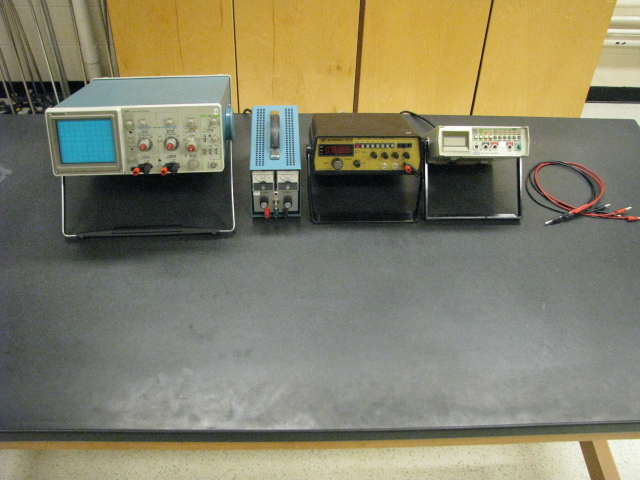
\includegraphics{AC-Measurements-Setup.jpg}
\caption{A photograph of the experimental setup.}
\label{fig:ACsetup}
\end{marginfigure}

\section{{\bf Preparation}}
% copy and paste the section under preparation (or similar section)
Review the properties of sine waves and the Root-Mean-Square value of a function.

\section{{\bf Goals of the Experiment}}
% copy and paste the section under goals of the experiment (or similar section)
\begin{itemize}
    \item To learn how to measure DC and AC voltage with a multimeter and an oscilloscope.
    \item To be able to measure peak-to-peak voltage (V$_{pp}$), peak voltage (V$_p$), average voltage (V$_{avg}$), RMS voltage (V$_{rms}$), and the period of time varying signals.
    \item To make connections between oscilloscope measurements and multimeter measurements.
\end{itemize}
%To learn to measure DC and AC voltage with a multimeter and an oscilloscope as well as be able to measure peak-to-peak voltage (V$_{pp}$), peak voltage (V$_p$), average voltage (V$_{avg}$), RMS voltage (V$_{rms}$), and the period of time varying signals. To understand which of these voltage measures is used by multimeters.

\section{{\bf Theory}}
Almost all devices operate and communicate using time-varying electrical signals and therefore, the ability to measure the properties of these signals (amplitude, time variation, etc.) is critical. This experiment gives practice and experience in making these measurements. The theory of DC (signals that do not vary in time) measurements, AC (signals that are time varying) measurements, and AC with DC (signals) measurements is presented in sections I, II, and III respectively. The DC signals are generated with a power supply while AC signals are generated with a function generator, which is explained in section IV. These signals are all measured with a standard multimeter as well as an oscilloscope, which is explained in sections V and VI.

\section{{\bf I - DC Voltage Measurements}}

\begin{marginfigure}
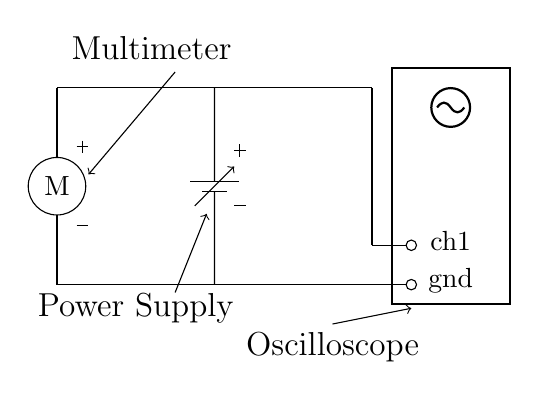
\begin{tikzpicture}[circuit ee IEC]
\draw(0,3) to (4,3);
\draw(4,3) to (4,1);
\draw(4,1) to (4.5,1);
\draw(0,.5) to (4.5,.5);
\draw(0,.5) to (0,3);
\draw[thick](4.25,.25) rectangle (5.75,3.25); % oscilloscope
\draw(2,3) to [battery](2,.5); %battery wire
\draw(2.25,1.5) to (2.4,1.5); %negative battery
\draw(2.25,2.2) to (2.4,2.2); %positive battery
\draw(2.32,2.28) to (2.32,2.12); %positive battery
\node[black,fill=white,draw=black,shape=circle,scale=1] at (0,1.75) {M}; % multimeter
\draw[->](1.75,1.5) to (2.25,2);
\node[black,fill=white,draw=black,shape=circle,scale=.4] at (4.5,.5) {}; %node
\node[black,fill=white,draw=black,shape=circle,scale=.4] at (4.5,1) {}; %node
\draw(.25,1.25) to (.4,1.25); %negative meter
\draw(.25,2.25) to (.4,2.25); %positive meter
\draw(.32,2.33) to (.32,2.17); %positive meter
\node at (5,1.05) {ch1};
\node at (5,.55) {gnd};
\node[ac source,thick] at (5,2.75){}; %oscilloscope symbol

%labels
\node at (1.2,3.5) {\large Multimeter};
\draw[thin,->] (1.5,3.2) to (.4,1.9);
\node at (1,.2) {\large Power Supply};
\draw[thin,->] (1.5,.4) to (1.9,1.4);
\node at (3.5,-.3) {\large Oscilloscope};
\draw[thin,->] (3.5,0) to (4.5,0.2); 

\end{tikzpicture}
\caption{Measuring DC power supply with oscilloscope and multimeter.}
\label{fig:acDCoscilloscope}
\end{marginfigure}


A multimeter is a good choice for measuring a steady voltage, such as that across the terminals of a power supply, but an oscilloscope can also be used, provided that great accuracy is not required. It is instructive to measure the terminal voltage of a power supply with both a multimeter and an oscilloscope and compare results as in Figure \ref{fig:acDCoscilloscope}.

As the output voltage of the power supply is increased it can be seen that the multimeter will give a non-zero reading, and that the horizontal line on the oscilloscope will move vertically. Both the reading on the multimeter and the displacement of the trace represent the voltage provided by the power supply. Note that the oscilloscope trace  only moves when the input coupling control is set to DC. In AC coupling mode the DC component of the input signal is blocked and the trace will remain stationary. The oscilloscope only measures voltage, so when current is being measured it should be removed from the circuit.


\section{{\bf II - AC Voltage Measurements}}
An oscilloscope is most useful when measuring time varying signals. Replace the power supply in the circuit with a sine function generator as seen in Figure \ref{fig:acACoscilloscope}. The multimeter reading can now be compared to the oscilloscope display. The trace on the crt display is, of course, a sine wave whose equation is given by

\begin{equation}
V(t)=V_0 sin(\omega t)=V_0sin(2\pi ft)=V_0sin\left(\frac{2\pi}{T}t\right)
\label{equ:ac1}
\end{equation}

\begin{marginfigure}
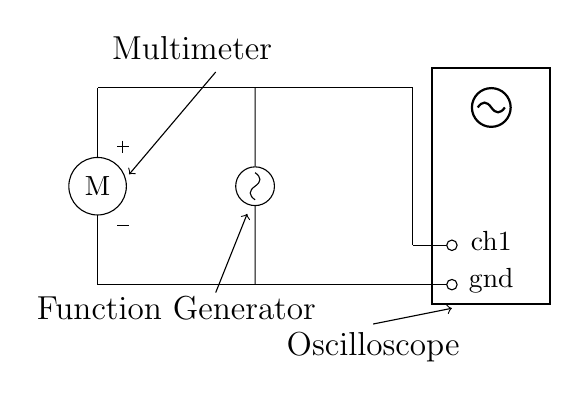
\begin{tikzpicture}[circuit ee IEC]

\draw (2,.5) to [ac source](2,3); %AC Source
\draw(0,3) to (4,3);
\draw(4,3) to (4,1);
\draw(4,1) to (4.5,1);
\draw(0,.5) to (4.5,.5);
\draw(0,.5) to (0,3);
\draw[thick] (4.25,.25) rectangle (5.75,3.25); % oscilloscope
\node[black,fill=white,draw=black,shape=circle,scale=1] at (0,1.75) {M}; % multimeter
\node[black,fill=white,draw=black,shape=circle,scale=.4] at (4.5,.5) {}; %node
\node[black,fill=white,draw=black,shape=circle,scale=.4] at (4.5,1) {}; %node
\draw(.25,1.25) to (.4,1.25); %negative meter
\draw(.25,2.25) to (.4,2.25); %positive meter
\draw(.32,2.33) to (.32,2.17); %positive meter
\node at (5,1.05) {ch1};
\node at (5,.55) {gnd};
\node[ac source,thick] at (5,2.75){}; %oscilloscope symbol

%labels
\node at (1.2,3.5) {\large Multimeter};
\draw[thin,->] (1.5,3.2) to (.4,1.9);
\node at (1,.2) {\large Function Generator};
\draw[thin,->] (1.5,.4) to (1.9,1.4);
\node at (3.5,-.3) {\large Oscilloscope};
\draw[thin,->] (3.5,0) to (4.5,0.2);


\end{tikzpicture}
\caption{Measuring AC power supply with oscilloscope and multimeter.}
\label{fig:acACoscilloscope}
\end{marginfigure}

\noindent where $\omega$ is the {\bf angular frequency} (in radians/second), f is the {\bf frequency} (in Hertz), and T is the {\bf period} (in seconds).

There are four ways of describing the height or amplitude of such a wave. These different {\bf amplitudes} can be seen in the sine wave shown in Figure \ref{fig:acSine}.

a) The peak value V$_p$ is the maximum voltage of the waveform. For the sine wave given by Equation \ref{equ:ac1} this  corresponds to V$_0$.

b) The peak to peak value V$_{p-p}$ is the full voltage difference between maximum and minimum values of the voltage. For the sine wave given by Equation \ref{equ:ac1} this equals 2V$_0$.

c) The average value V$_{av}$ over half a period. This value is found from the equation

\begin{equation}
V_{avg}=\frac{2}{T}\int\limits_{0}^{T/2}V(t)dt=\frac{2}{T}\int\limits_{0}^{T/2}V_0sin(\omega t) dt=\frac{2V_0}{\pi}\approx 0.637V_0
\label{equ:ac2}
\end{equation}


\begin{figure}%[h,scale=.7]
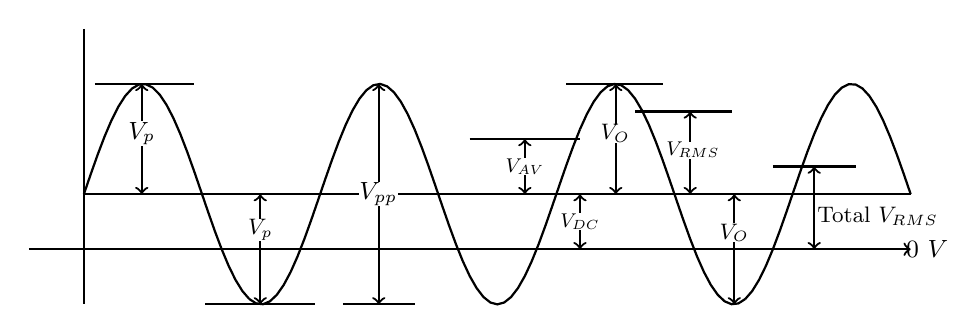
\begin{tikzpicture}[scale=.7,font=\small,inner sep=0]
\draw[thick] (0,4)--(0,-1); %yaxis
\draw[thick,->](-1,0)--(15,0); %xaxis

%broken up domain needed for smoothness
\draw[thick,domain=0:3] plot (\x,{2*sin(\x*84)+1}); %sine
\draw[thick,domain=3:6] plot (\x,{2*sin(\x*84)+1}); %sine
\draw[thick,domain=6:9] plot (\x,{2*sin(\x*84)+1}); %sine
\draw[thick,domain=9:12] plot (\x,{2*sin(\x*84)+1}); %sine
\draw[thick,domain=12:15] plot (\x,{2*sin(\x*84)+1}); %sine
\draw[thick](0,1)--(15,1); %middle line
\draw[thick](0.2,3)--(2,3); %first horiz line
\draw[thick](2.2,-1)--(4.2,-1); %second horiz line
\draw[thick](4.7,-1)--(6,-1); %third horiz line
\draw[thick](7,2)--(9,2); %fourth horiz line
\draw[thick](8.75,3)--(10.5,3); %5th horiz line
\draw[thick](10,2.5)--(11.75,2.5); %6th horiz line
\draw[thick](12.5,1.5)--(14,1.5); %last horiz line

\node[thick] at (15.3,0) {0 $V$}; %0 Volts label
\draw[thick,<->](1.05,1)--(1.05,3); %V_p
\node[black,fill=white,draw=white,shape=rectangle,scale=1] at (1.05,2.1) {$V_p$}; %V_p label
\draw[thick,<->](3.2,1)--(3.2,-1); %V_p
\node[black,fill=white,draw=white,shape=rectangle,scale=.9] at (3.2,.35) {$V_p$}; %V_p label
\draw[thick,<->](5.35,-1)--(5.35,3); %V_pp
\node[black,fill=white,draw=white,shape=rectangle,scale=1] at (5.34,1) {$V_{pp}$}; %V_pp label
\draw[thick,<->](8,1)--(8,2); %V_av
\node[black,fill=white,draw=white,shape=rectangle,scale=.8] at (8,1.5) {$V_{AV}$}; %V_av label
\draw[thick,<->](9,1)--(9,0); %V_dc
\node[black,fill=white,draw=white,shape=rectangle,scale=.8] at (9,.5) {$V_{DC}$}; %V_dc label
\draw[thick,<->](9.65,1)--(9.65,3); %V_o
\node[black,fill=white,draw=white,shape=rectangle,scale=.9] at (9.64,2.1) {$V_O$}; %V_o label
\draw[thick,<->](11,1)--(11,2.5); %V_rms
\node[black,fill=white,draw=white,shape=rectangle,scale=.8] at (11.05,1.8) {$V_{RMS}$}; %V_rms label
\draw[thick,<->](11.8,1)--(11.8,-1); %V_o
\node[black,fill=white,draw=white,shape=rectangle,scale=.9] at (11.8,.3) {$V_O$}; %V_o label
\draw[thick,<->](13.25,1.5)--(13.25,0); %total V_rms
\node[black,fill=white,draw=white,shape=rectangle,scale=.9] at (13.3,.6) [right]{Total $V_{RMS}$}; %V_rms label
\end{tikzpicture}
\caption{The four ways of defining the amplitude of a sine wave.}
\label{fig:acSine}
\end{figure}



d) The effective or {\bf r}oot {\bf m}ean {\bf s}quare (RMS) value, Vrms, is defined as the equivalent dc voltage that will supply the same power, P, to a resistance, R, as the original waveform over a full period. So

\begin{equation}
P=\frac{1}{T}\int\limits_{0}^{T}\frac{V^2(t)}{R}dt=\frac{1}{T}\int_{0}^{T}\frac{V_0^2}{R}sin^2(\omega t) dt=\frac{V_0^2}{2R}
\label{equ:ac3}
\end{equation}

By the above definition, the rms voltage is that dc voltage which would supply the same power to the resistor. Therefore

\begin{equation}
P=\dfrac{V_{rms}^2}{R}=\frac{V_0^2}{2R}
\label{equ:ac4}
\end{equation}

\noindent and thus

\begin{equation}
V_{rms}=\sqrt{RP}=\sqrt{\frac{1}{T}\int_{0}^{T}V^2(t)dt}=\sqrt{\frac{1}{T}\int_{0}^{T}V_0^2sin^2\omega tdt}=\frac{V_0}{\sqrt{2}}\approx 0.707V_0
\label{equ:ac5}
\end{equation}

\section{{\bf III - AC and DC Measurements}}

The offset control on the function generator can be used to add a DC component to the output waveform. This can be seen in Figure \ref{fig:acSine} where the sine wave is offset vertically. The sine wave can be observed to move up and down on the oscilloscope when the offset control is adjusted. As with the power supply, one can see that the trace will only move when the input controls are set to DC coupling. With AC coupling the DC level is removed and only the sine wave appears on the screen. Similarly, when the multimeter is set to read AC volts or amps, only the AC component is measured. When the multimeter function is DC volts or amps, only the DC level is measured.

The equation of a sine wave together with a DC level is given by

\begin{equation}
V(t)=V_0sin(\omega t)+V_{DC}
\label{equ:ac6}
\end{equation}

Here, the frequency is the same as in Equation \ref{equ:ac1} but the amplitude is different. The sine wave with extra DC component would supply more power to a resistor than the sine wave alone. For the case of a waveform riding on top of a DC level, the rms amplitude is given by the formula

\begin{equation}
Total \hspace{1mm} V_{rms}=\sqrt{(ac\hspace{1mm} rms\hspace{1mm} component)^2+V_{DC}^2}
\label{equ:ac7}
\end{equation}

For the sine wave in Equation \ref{equ:ac6} this formula reduces to

\begin{equation}
Total \hspace{1mm} V_{rms}=\sqrt{\frac{V_0^2}{2}+V_{DC}^2}
\label{equ:ac8}
\end{equation}

Figure \ref{fig:acSine} shows a sinewave riding on a DC level with the various different amplitudes labeled.






\section{{\bf IV - The Function Generator}}

The function generator is an instrument that generates time varying electrical signals. Front panel controls set the shape, size, rate, and other properties of the output waveform. The B\&K 3011 can generate sine waves, triangle waves, and rectangular waves.

Before connecting the function generator into a circuit, it is essential to make sure that it has been properly configured for the appropriate output signal. Standard practice is to use an oscilloscope to view the output of the function generator directly. Once the wave form is correctly displayed on the screen, the function generator is powered off and connected to the circuit. Do {\bf not} connect an operating function generator to a circuit as it is being wired together. When the circuit wiring is completed, the function generator is powered up, along with any other power supplies and sources that the circuit needs. The function generator {\bf cannot} withstand a short circuit across the output terminals. Always check the circuit you are driving with the function generator to make sure that the output is not being shorted out.

Figure \ref{fig:acFG} shows the operating controls of the function generator. When setting up this instrument, the first task is to choose the appropriate shape (sine, square, or triangle) using the three {\bf FUNCTION} buttons. The waveform appears at the connector labeled {\bf OUTPUT}. The other two output jacks are not commonly used. Secondly, adjust the amplitude of the signal by adjusting the knob labeled {\bf AMPL} to about one quarter of the way between {\bf min} and {\bf max}. The buttons labeled {\bf DUTY}, {\bf OFFSET}, {\bf TTL}, and {\bf AMPL} must all be pushed in. Pulling them out changes the range or adds other functions. The left knob of these four (DUTY) changes the symmetry of the waveform. Make sure this knob is rotated fully counterclockwise to the CAL position. If it is not in the proper position, some output waveforms will appear distorted.

Lastly, it remains to set how often the waveform repeats itself. The push buttons labeled 1, 10, 100, 1K, 10K, 100K, and 1M set the {\bf range} of the repetition rate. Inside any given range the repeat rate is set by the {\bf COARSE} and {\bf FINE} controls. For sine waves these controls adjust the {\bf frequency} of the wave. For triangle waves and rectangle waves, frequency is not an accurate description and the term {\bf repetition rate} is used instead. 

\begin{figure}
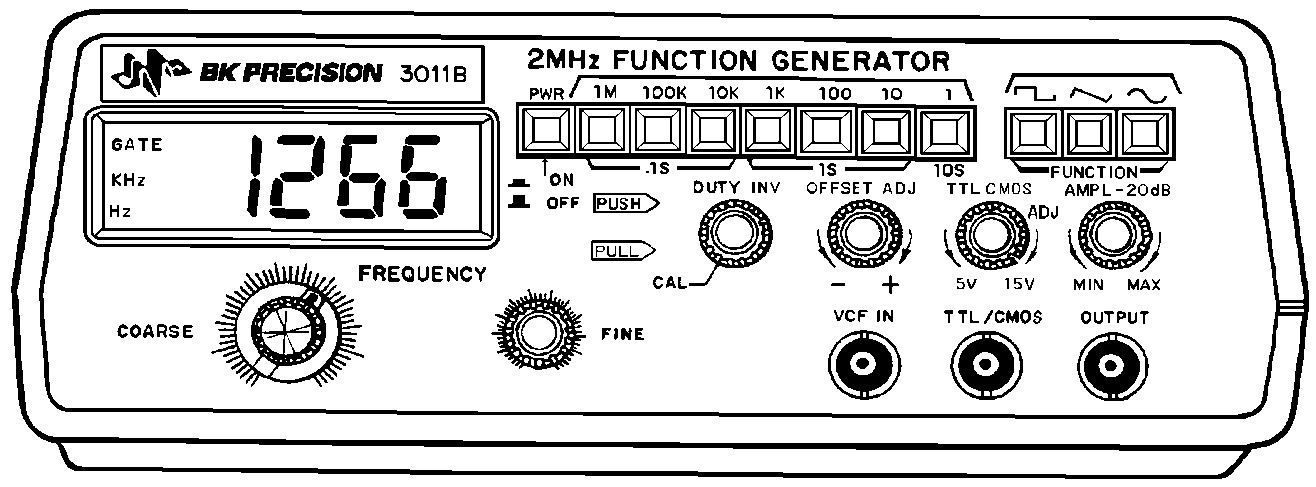
\includegraphics{AC-Measurements-func-gen.png}
\caption{BK 3011B function generator control panel.}
\label{fig:acFG}
\end{figure}

\section{{\bf V - The Oscilloscope}}

An oscilloscope is an instrument which usually displays a graph (trace) of the voltage of a signal plotted against time. Time is plotted horizontally, in the x-direction and voltage is plotted vertically, in the y-direction. The graph changes as the voltage changes, so both the waveform and any changes in the waveform can be monitored. Both the voltage scale and the time scale can be adjusted over several orders of magnitude. Measurements of voltages and times can be made by comparing the trace with the transparent scale mounted in front of the screen on which the trace appears. 

The trace is formed by the motion of a bright spot which appears where a narrow electron beam hits the phosphor on the screen of a cathode ray tube (CRT). The electron beam can be deflected in the x and y directions by the electric field caused by amplified signals applied to deflector plates inside the tube. These amplified signals are generated inside the oscilloscope in response to controls the operator sets as well as the actual waveform to be measured. Details of how the CRT works can be found in most books on electricity and magnetism.

\section{{\bf Oscilloscope Controls}}

Even the simplest oscilloscope has several controls, all of which must be set within fairly narrow limits in order to give a good trace. More advanced instruments have additional features and controls which will not be mentioned here. Many oscilloscopes provide dual traces, so that two waveforms can be viewed simultaneously. This makes it easy to compare two signals. Figure \ref{fig:acOscilloscope} shows the controls of a typical oscilloscope.

\begin{figure}
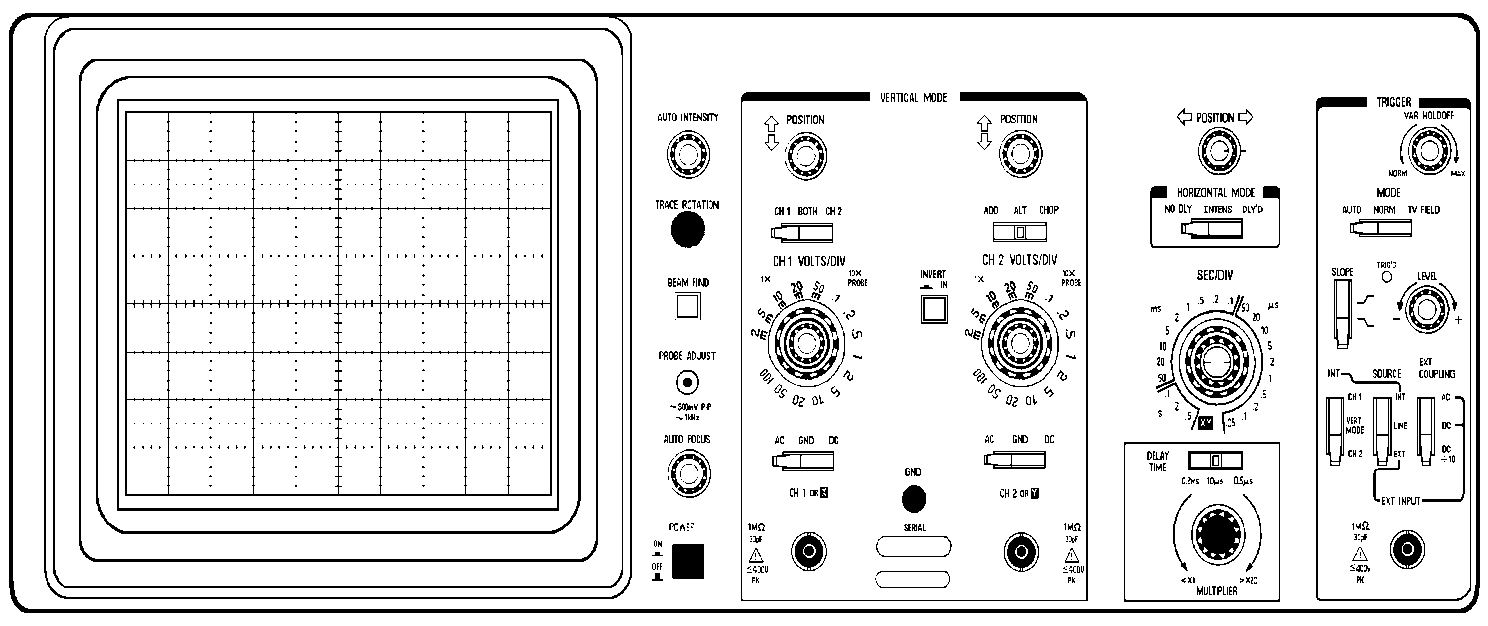
\includegraphics{AC-Measurements-osc-controls.png}
\caption{Oscilloscope display panel.}
\label{fig:acOscilloscope}
\end{figure}

\begin{enumerate}
\item Basic display controls

(a) {\bf Focus} This controls the size of the spot on the screen, and thus sharpness of the trace which forms the graph. It should be adjusted to give a clear fine image.

(b) {\bf Intensity} This controls the brightness of the spot. If the spot is too dim the Trace is too faint to see. A trace which is too bright will eventually leave a permanent mark on the screen, and in any case tends to smear the trace and hide details. It is good practice to use the lowest intensity that will show all the necessary detail in the trace without straining the eyes.

\item Position controls

These control the horizontal and vertical position of the trace. Usually only small changes are necessary in the horizontal position of the trace. Quite large adjustments may be needed for the vertical position. If no trace is visible on the screen, reduce the vertical gain (see below) or ground the signal using the input coupling controls. Then make sure that the intensity is not too low, and set the x and y position controls to the middle of their range. This will usually bring the spot onto the screen. It may be that the time base is not triggering (see below). Some oscilloscopes have a "beam find" button which can be pushed to locate the trace if it is off screen. This can be a useful time saver.

\item Vertical Gain

The vertical scale of the display is set by the vertical gain control, usually a multi-position rotary switch. The scale is usually given in V/cm (or mV/cm). A dual trace oscilloscope has two independent sets of controls, one for each channel. They are often labeled "Channel A" and "Channel B" or "Channel 1" and "Channel 2". If a continuous control is provided, usually a small knob in the center of the rotary switch, make sure it is turned completely to the "CAL" position before making any measurements.

\item Coupling Controls

The input signal can be connected ("coupled") to the amplifier for the vertical channel(s) either directly (DC coupling) or through a capacitor (AC coupling). A third possibility is to ground the input of the amplifier, which provides a quick way of finding the zero signal position of the trace. AC coupling blocks any DC component of the signal. This is useful when a varying signal is superimposed on a steady voltage, and one wants to zoom in to examine the varying part in detail. If the steady part of the signal needs to be examined then DC coupling is required.

\item Time base

The time base or sweep moves the spot horizontally to the right at a controlled speed, then returns it rapidly to the left of the screen to start again. The sweep or time-base sets the horizontal scale of the display, and is typically controlled by a multi-position rotary switch. The scale is given in s/cm, ms/cm, $\mu$s/cm, and ns/cm. there may be a knob at the center of the rotary switch which gives a continuous change of scale, but which clicks to a preset "calibrated" setting when turned to the far left or right. This control must be in the "calibrated position" before making any measurements of time intervals. It is good practice to check the appearance of the signal at a wide range of time-base settings before starting to make measurements. Some features are best seen at slow speeds while others may show up better at high speeds.

\item Triggering

This controls the time at which the sweep starts. For the display to be steady the sweep should start at the same point on a repetitive signal every time the sweep begins. In this way successive traces will be in the same position.

(a) {\bf Trigger Source} The choices are usually INT ( an internally generated signal being supplied to the horizontal amplifier), EXT (some external signal source), and LINE (the 60Hz line frequency). For most purposes INT is the correct choice. Some signal generators have a SYNC output signal which can be used to trigger the oscilloscope using EXT. The LINE trigger source is used for observing signals that are related to the AC power line. If there is a trigger mode control usually the AUTO setting is the correct one. With dual trace oscilloscopes make sure the trigger source is the appropriate channel. A channel with no signal will give poor triggering.

(b) {\bf Trigger Level} This sets the signal voltage value at which the sweep starts. If an AUTO mode is available try it. If this gives a good trace use that setting. If the AUTO does not give a good trace, usually some experimentation is needed, especially with the LEVEL control. If the LEVEL setting is too low, the sweep will trigger at several different points in the waveform, and the successive traces will not overlap properly, giving an unstable messy display. If the level is set too high, the sweep may not trigger at all, and there will be no trace, or only a dot on the left. One often has to experiment quite a lot to get a good stable trace with certain types of signal. Remember to check that the source of the trigger is the same as the signal you are actually looking at and trying to stabilize. Sometimes the trigger level has to be set carefully at one particular position to give a good stable trace, so perseverance is needed

(c) {\bf Trigger Slope} One can choose whether the sweep will start with a positive- or negative- going  part of the signal. Note that a trigger level alone is not enough to uniquely determine a position on a repetitive signal. The slope at that point must be set as well.
\end{enumerate}

\section{{\bf Experimental Procedure}}

\begin{enumerate}
\item Set up the circuit shown in Figure \ref{fig:acDCoscilloscope}. Make sure the power supply is initially set to zero volts (voltage knob fully counter-clockwise) and the current knob is turned fully clockwise. Turn on both the oscilloscope and the multimeter. Set up the multimeter to measure DC voltages. Select ranges on both the scope and multimeter for a maximum of approximately 10 to 20 volts. Set the scope to DC coupling so that DC levels can be observed. For at least four different DC voltage levels, measure the output of the power supply with both the multimeter and the oscilloscope.

\item Set up the circuit shown in Figure \ref{fig:acACoscilloscope}. Connect the multimeter as a voltmeter. Select the sine function on the generator and a frequency of about 1 kHz. To obtain a stationary trace on the scope you will have to adjust both your time base and the frequency. A single period should almost fill the whole screen. Make sure the time base and the vertical gain are both in their calibrated positions or else the numbers you obtain will be incorrect. Make a sketch of what is observed on the oscilloscope screen.

\item For at least four frequencies between 100Hz and 1MHz, measure the frequency of the function generator with both the oscilloscope and the function generator panel meter.

\item The amplitude of the sine wave can be measured with both the multimeter and the oscilloscope and compared. Configure the multimeter for measuring AC voltage. The oscilloscope is naturally suited for measuring the peak-to-peak amplitude of a signal. From this the peak, average, and rms amplitudes can be derived. The point of this step is to deduce which kind of amplitude the multimeter reports. For at least four different amplitudes, measure the amplitude of the sine wave using both the oscilloscope and multimeter. Each of the four sine waves should have a different frequency as well. For best results keep the frequency between 100Hz and 20kHz. 

\item The function generator is not restricted to generating sine waves. It can also generate square waves. For four different amplitudes of a 1kHz square wave, measure the peak and rms voltage of the square wave, using the oscilloscope and multimeter.

\item Note that the DC offset control on the function generator adds a DC level to the output waveform. This suggests that readings can be compared between the multimeter and the oscilloscope for the total rms voltage of a signal with both DC and AC components. For four different amplitudes and DC offsets of a 5kHz sine wave, measure the total rms voltage using both the multimeter and the oscilloscope. It will be necessary to make two measurements with each instrument, one for the DC component and one for the AC component.

\item Determine whether the oscilloscope screen plots from left to right or from right to left. Detail the observations that support your claim.

\item Oscilloscopes can respond to much higher frequencies than multimeters can. Measure the voltage of a sine wave with a multimeter and then increase the frequency until the multimeter has difficulty reporting a voltage. Record how the multimeter and oscilloscope react differently at this frequency.
\end{enumerate}


\section{{\bf Error Analysis}}

The accuracy of digital meters is generally better than that of typical analog meters, but there is always some uncertainty in the calibration of any instrument. Good quality multimeters will have a statement about their accuracy in the instruction manual, or more conveniently, on the case of the instrument itself, typically on the bottom. Suppose now that we have selected the DC current function along with the 200 mA range. The reading is 98.6 mA and we want to find the uncertainty in the reading. To obtain the required information we look on the bottom face of the meter where there is printed information regarding the uncertainty of the various ranges. In the second line we read "DC current  (0.3 + 1)". The +1 inside this bracket means that the last digit in the reading could be any one of 5, 6, or 7 and, hence, that the actual current could be anywhere in the interval

\begin{equation}
98.5\leq I \leq 98.7
\label{equ:ac9}
\end{equation}

The 0.3 indicates that there is an uncertainty of 0.3 \% in the reading due to calibration errors. Taking the worst case (always), we compute the calibration uncertainty in the reading,  I$_C$  as

\begin{equation}
u(I_C)=0.003\times98.7mA=0.3mA
\label{equ:ac10}
\end{equation}

\begin{equation}
98.5-0.3\leq I\leq 98.7+0.3mA
\label{equ:ac11}
\end{equation}

\begin{equation}
I=98.6\pm 0.4mA
\label{equ:ac12}
\end{equation}

\begin{equation}
u(I)=0.4mA
\label{equ:ac13}
\end{equation}

This is the procedure to be followed for computing the uncertainty in any reading made with this multimeter.

The voltage scale and time scale of the oscilloscope both have a calibration uncertainty of 3\%. There is also a reading error of 4\% (half of the smallest division on the screen). Combining these two uncertainties in quadrature results in a measurement error for the oscilloscope of 5\%. This error must be applied for both time measurements (horizontal) and voltage measurements (vertical). The procedure to be followed to compute the uncertainty in any reading made with the oscilloscope is to add an error of 5\% of full scale (not the reading!). This is equivalent to one-half of a major division (or 2.5 times a minor division) for the time scale and a good approximation to one-half of a major division for the voltage scale. Note that this uncertainty is much higher than that of the multimeter.

The digital frequency readout on the function generator has an associated uncertainty of $\pm 1$ digit.

\section{{\bf To be handed in to your lab instructor}}

%%% begin prelab %%%
\section{{\bf Prelab}}
\begin{enumerate}
\item AC: Show that the rms amplitude of a square wave is the same as the peak value of the square wave.

\item When measuring a voltage the multimeter scale setting can be set to the 0.2V, 2V, 20V, or 200V range. This is the maximum voltage the multimeter can reliably measure on that setting. What is the most appropriate multimeter scale setting to use when measuring voltages of 1.5V, 10V, and 30V? See the error analysis section of this lab and think about the uncertainty that would be associated with each measurement.
 
\item When measuring a voltage the oscilloscope vertical gain can be set to the 0.1V, 0.2V, 0.5V, ..., 5V, 0r 10V range. What is the most appropriate oscilloscope vertical gain to use when measuring voltages of 0.05V, 0.15V, 0.2V?

\item An oscilloscope measures the two quantities voltage and time. Therefore, is it possible to directly measure the frequency of a voltage signal with an oscilloscope or is the frequency calculated from another measurement? 
\end{enumerate}
%%% end prelab %%%

\section{{\bf Data Requirements}}
\begin{enumerate}[resume]
\item DC: A table of voltage measurements from the multimeter and the oscilloscope for four different voltage settings of the power supply with uncertainties (Procedure step 1).

\item AC: A sketch of a sine wave, for one frequency and one amplitude, as it appears on the oscilloscope screen. Clearly indicate T, $V_{p-p}$, V$_p$, V$_{avg}$, and $V_{rms}$ on the graph. Also indicate the major oscilloscope graticule lines and the vertical and horizontal oscilloscope scales used (Procedure step 2).

\item AC: A table of frequency measurements together with uncertainty from the function generator and period of the waveform together with uncertainty as measured using the oscilloscope for four different sine waves, with frequencies between 100 Hz and 1 MHz (Procedure step 3).

\item AC: A table of voltage measurements for four different sine waves, with different frequencies between 100Hz and 20kHz, measured with the the multimeter and the oscilloscope (Procedure step 4). Include the multimeter amplitude, oscilloscope peak voltage, oscilloscope peak to peak voltage, calculated oscilloscope rms voltage, and calculated oscilloscope average voltage.
 
\item AC: A table of voltage measurements for four different amplitudes of a 1 kHz square wave measured with the multimeter and the oscilloscope (Procedure step 5).

\item DC and AC: A table of voltage measurements of a 5 kHz sine wave for four different amplitudes and DC offsets measured with the multimeter and oscilloscope (Procedure step 6). Include the multimeter DC voltage, RMS AC voltage, total RMS voltage, and oscilloscope DC voltage, peak AC voltage component, RMS AC voltage, and total RMS voltage.

\item Observations indicating whether the oscilloscope plots from left to right or right to left (Procedure step 7).
 
\item Observations of the multimeter and oscilloscope behaving at high frequencies (Procedure step 8).
\end{enumerate}


\section{{\bf Discussion}}
\begin{enumerate}[resume]
\item DC: Compare the voltage readings of the multimeter and oscilloscope for the four different voltage settings of the power supply. Include the measurement uncertainties.

\item AC: For the four different sine waves with frequencies between 100 Hz and 1 MHz, compare the frequency reading on the function generator with the frequency of the waveform as measured using the oscilloscope. Fill in a table with the function generator frequency, oscilloscope period, oscilloscope frequency, and error in the oscilloscope frequency.

\item AC: For the four different amplitudes of sine waves, with frequencies between 100 Hz and 20 kHz, measured using the multimeter and the oscilloscope, fill in a table with the multimeter RMS voltage, and calculated oscilloscope peak voltage, oscilloscope peak to peak voltage, calculated oscilloscope RMS voltage, and calculated oscilloscope average voltage.

\item AC: For the four different amplitudes of a 1 kHz square wave, fill in a table with the amplitude using both the scope and the multimeter.

\item DC and AC: For the four different amplitudes and offsets of a 5 kHz sine wave and square wave, fill in a table with the multimeter DC voltages, RMS AC voltages, total RMS voltage, and oscilloscope DC voltage, peak AC voltage component, RMS AC voltage, and total RMS voltage.
\end{enumerate}


\AtEndDocument{\clearpage\ifodd\value{page}\else\null\clearpage\fi} % forces even page count, for double siding


%%%end document%%% DO NOT REMOVE THIS LINE

%%%start companion guide%%% DO NOT REMOVE THIS LINE
\chapter{AC Measurements - Companion Guide}

\section{Equipment}

% first column
\begin{minipage}[t]{0.55\textwidth}
\begin{itemize}[noitemsep]
\item Fluke multimeter
\item Oscilloscope
\item Anatek power supply
\end{itemize}
\end{minipage}
%second column
\begin{minipage}[t]{0.45\textwidth}
\begin{itemize}[noitemsep]
\item B$\And$K 3011 function \\generator
\item set of connecting leads (2)
\end{itemize}
\end{minipage}


\section{Setup}
\begin{figure}
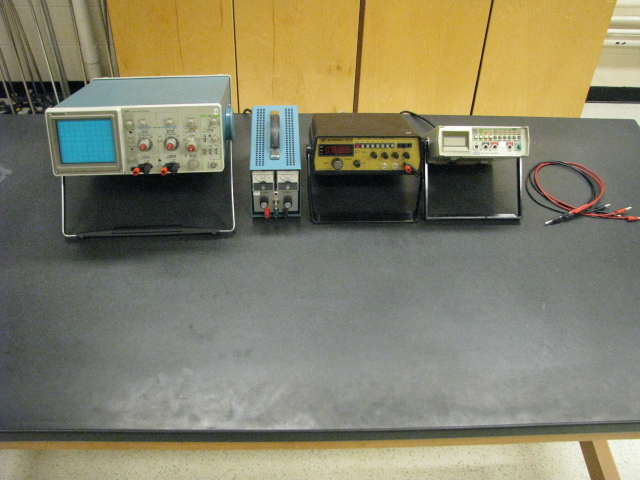
\includegraphics{AC-Measurements-Setup.jpg}
\caption{Equipment Setup}
\label{pic:ACsetup}
\end{figure}

Set up bench as shown in Figure \ref{pic:ACsetup}.

\section{Maintenance}

\begin{enumerate}
\item 
\item 
\end{enumerate}

\section{Critical Points of Failure}

There are currently no known critical points of failure.

\section{Notes to the Instructor}
\begin{enumerate}
\item All connections should be made while the power is off.
\item Students should record the sec/div and V/div off the oscilloscope for all measurements so that uncertainties can be calculated in the discussion section.
\item Students may be confused with instructions that ask them to measure rms voltage off the oscilloscope. Peak-to-peak voltage is measured off the screen and must then be converted to the rms voltage.
\item Procedure step 6 requires that students adjust both the amplitude and DC level of an AC signal. It is important to note that the maximum output voltage of the function generator is approximately $\pm14$ V. This means that students should work with appropriate voltages to avoid having their signal flatten out at the top or bottom.
\item For procedure step 6, students may be confused about what they are measuring from which device. They will read the rms AC voltage and DC voltage level straight from the AC and DC settings on the multimeter. On the oscilloscope, students will first measure the peak-to-peak voltage, as before, using the AC-coupling setting. Then they must adjust the trace so that either a peak or a trough is lined up with one of the major divisions on the screen. It is convenient to line up a peak with the x-axis. Then they will switch to the DC-coupling setting and measure the displacement of the peak. This value is the DC level. They will then use these values to calculate the total rms voltage.
\end{enumerate}

\section{Prelab Questions}

These are example answers and derivations to the prelab questions. They are not necessarily the only possible derivations or answers.

\begin{enumerate}
\item {\bf AC: Show that the rms amplitude of a square wave is the same as the peak value of the square wave.}\newline

We need to show that $V_{rms}=V_{p}$, given the square wave shown in Figure \ref{fig:accg1}. 

\begin{marginfigure}
\begin{tikzpicture}
%\draw[](0,0)rectangle(6,5);
\draw[very thin,->](0,2.5)--(5,2.5);
\draw[very thin,<->](0,1)--(0,4);
\draw[](0,3.5)--(1.5,3.5)--(1.5,1.5)--(3,1.5)--(3,3.5)--(4.5,3.5);
%labels
\node[font=\small]at(-.25,3.5){$V_p$};
\node[font=\small]at(3.2,2.3){T};
\end{tikzpicture}
\caption{A square wave with 50\% duty cycle.}
\label{fig:accg1}
\end{marginfigure}

%\begin{align*}
\begin{subequations}
\begin{equation}
V_{rms}=\sqrt{\dfrac{1}{T}\int\limits_{0}^{T}V(t)^2dt}
\end{equation}
\begin{equation}
=\sqrt{\dfrac{1}{T}\int\limits_0^{T/2}(V_p)^2dt+\int\limits_{T/2}^{T}(-V_p)^2dt}
\end{equation}
\begin{equation}
=\dfrac{V_p}{\sqrt{T}}\sqrt{\left[t\right]_0^T}
\end{equation}
\begin{equation}
=\dfrac{V_p}{\sqrt{T}}\sqrt{T}
\end{equation}
\begin{equation}
=V_p
\end{equation}
\label{equ:accg1}
\end{subequations}
%\end{align*}

\item {\bf What is the most appropriate multimeter scale setting when measuring voltages of 1.5 V, 10 V, and 30 V?}\newline

Table \ref{tab:accg1} gives a summary of the determination of an appropriate voltage scale given that $u(V)=\pm 5\%$ for measurements made with the Fluke multimeter.

\begin{table}[ht]
\center
\begin{tabular}{|c|c|c|c|c|}\hline
V   & u(V)  & $V_{max}$ & $V_{min}$ & appropriate scale \\ \hline
1.5 & 0.075 & 1.575     & 1.425   & 2 V \\\hline
10  & 0.5   & 10.5      & 9.5     & 20 V \\\hline
30  & 1.5   & 28.5      & 31.5    & 200 V\\\hline
\end{tabular}
\caption{Results for question 2.}
\label{tab:accg1}
\end{table}


\item {\bf What is the most appropriate oscilloscope vertical gain to use when measuring voltages of 0.05 V, 0.15 V, and 0.2 V?}\newline

Table \ref{tab:accg2} gives a summary of the determination of an appropriate vertical gain. Given that we desire to minimize the uncertainty in our measurement, we should select a vertical gain that results in the trace filling as much of the screen as possible, as seen in Figure \ref{fig:accg2}.

\begin{marginfigure}[-20cm]
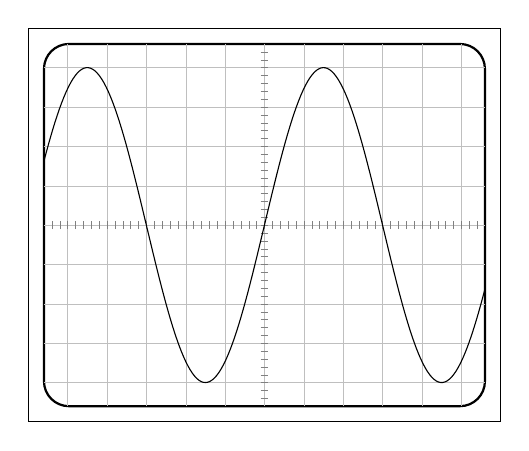
\begin{tikzpicture}
\draw[](0,0)rectangle(6,5);
\draw[rounded corners=9,thick](0.2,0.2)rectangle(5.8,4.8);
\draw[](3,.2)--(3,4.8);
\draw[](.2,2.5)--(5.8,2.5);
\foreach \x in {0,.5,...,5}{
\draw[ultra thin,draw=lightgray](.5+\x,.2)--(.5+\x,4.8);
}
\foreach \y in {0,.5,...,4}{
\draw[ultra thin,draw=lightgray](.2,.5+\y)--(5.8,.5+\y);
}
%tics
\foreach \x in {0,.1,...,5.5}{
\draw[ultra thin,draw=gray](.3+\x,2.45)--(.3+\x,2.55);
}
\foreach \y in {0,.1,...,4.5}{
\draw[ultra thin,draw=gray](2.95,.3+\y)--(3.05,.3+\y);
}
%function
\draw[domain=.2:5.8]plot [samples=200](\x,{2*sin(\x*120)+2.5});
\end{tikzpicture}
\caption{An appropriately filled oscilloscope screen.}
\label{fig:accg2}
\end{marginfigure}

\begin{table}[ht]
\center
\begin{tabular}{c|c}
V    & appropriate scale \\\hline
0.05 & 0.1 V \\
0.15 & 0.2 V \\
0.2  & 0.5 V
\end{tabular}
\label{tab:accg2}
\caption{Results for question 3.}
\end{table}

\item {\bf Is it possible to directly measure the frequency of a voltage signal with an oscilloscope or is the frequency calculated from another measurement?}\newline

The period of a sine wave may be read directly off an oscilloscope however the frequency must be calculated from that result. It may not be directly read off the oscilloscope.

\end{enumerate}


\section{Data Requirements}
\begin{enumerate}[resume]

\item {\bf DC: A table of voltage measurements from the multimeter and the oscilloscope for four different voltage settings of the power supply (Step 1).}\newline

\begin{table}[ht]
\center
\begin{tabular}{|l|l|}
\hline
$V_{mm}$ & $V_{osc}$ \\ \hline
1.90     & 2.1       \\ \hline
3.81     & 4.0       \\ \hline
12.57    & 13.0      \\ \hline
16.37    & 17.0      \\ \hline
\end{tabular}
\label{tab:accg3}
\end{table}

\item {\bf AC: A sketch of a sine wave, for one frequency and one amplitude, as it appears on the oscilloscope screen. Clearly indicate T, $V_{p-p}$, V$_p$, V$_{avg}$, and $V_{rms}$ on the graph. Also indicate the major oscilloscope graticule lines and the vertical and horizontal oscilloscope scales used (Procedure step 2).}\newline

\begin{figure}
\center
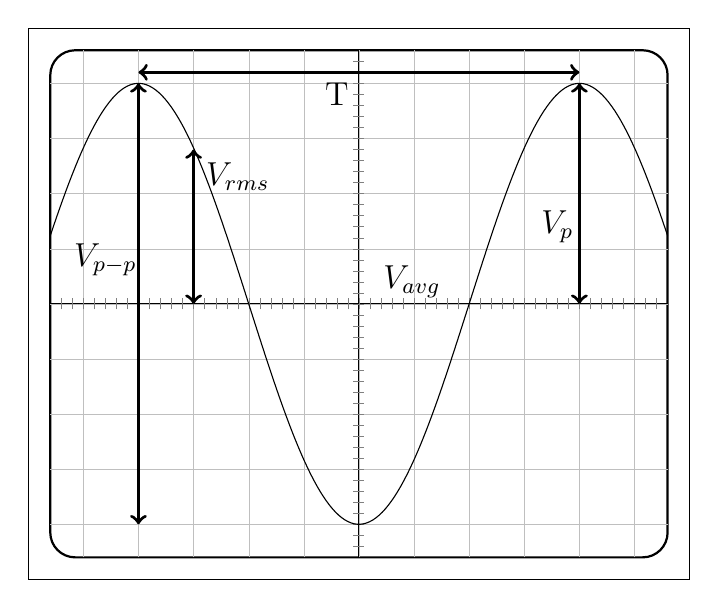
\begin{tikzpicture}[scale=1.4,inner sep=0]
\draw[](0,0)rectangle(6,5);
\draw[rounded corners=9,thick](0.2,0.2)rectangle(5.8,4.8);
\draw[line width=.5](3,.2)--(3,4.8);
\draw[line width=.5](.2,2.5)--(5.8,2.5);
\foreach \x in {0,.5,...,5}{
\draw[ultra thin,draw=lightgray](.5+\x,.2)--(.5+\x,4.8);
}
\foreach \y in {0,.5,...,4}{
\draw[ultra thin,draw=lightgray](.2,.5+\y)--(5.8,.5+\y);
}
%tics
\foreach \x in {0,.1,...,5.5}{
\draw[ultra thin,draw=gray](.3+\x,2.45)--(.3+\x,2.55);
}
\foreach \y in {0,.1,...,4.5}{
\draw[ultra thin,draw=gray](2.95,.3+\y)--(3.05,.3+\y);
}
%function
\draw[domain=.2:5.8]plot [samples=200](\x,{2*sin(\x*90)+2.5});
%labels
\draw[very thick,<->](1,4.6)--(5,4.6);
\node[font=\large]at(2.8,4.4){T};
\draw[very thick,<->](1,.5)--(1,4.5);
\node[font=\large]at(.7,2.9){$V_{p-p}$};
\draw[very thick,<->](5,2.5)--(5,4.5);
\node[font=\large]at(4.8,3.2){$V_{p}$};
\draw[very thick,<->](1.5,2.5)--(1.5,3.9);
\node[font=\large]at(1.9,3.65){$V_{rms}$};
\node[font=\large]at(3.48,2.7){$V_{avg}$};
\end{tikzpicture}
\caption{A sketch of a signal trace on an oscilloscope screen. As drawn, $V_{avg}$ is the x-axis.}
\label{fig:accg3}
\end{figure}

\item {\bf AC: A table of frequency measurements together with uncertainty from the function generator and period of the waveform as measured using the oscilloscope for four different sine waves, with frequencies between 100 Hz and 1 MHz (Procedure step 3).}\newline

A summary of the collected data from step 3.

\begin{table}[ht]
\center
\begin{tabular}{|l|l|l|l|l|}
\hline
\multicolumn{1}{|c|}{$f_{func gen}$ (Hz)} & \multicolumn{1}{c|}{$u(f)$} & \multicolumn{1}{c|}{T (s)} & \multicolumn{1}{c|}{u(T)} & \multicolumn{1}{c|}{sec/div} \\ \hline
101                                       & 1                           & 0.01                       & $1.00\times10^{-3}$       & $2.00\times10^{-3}$          \\ \hline
880                                       & 1                           & $1.15\times10^{-3}$        & $1.00\times10^{-4}$       & $2.00\times10^{-4}$          \\ \hline
2064                                      & 1                           & $4.80\times10^{-4}$        & $5.00\times10^{-5}$       & $1.00\times10^{-4}$          \\ \hline
95800                                     & 100                         & $1.04\times10^{-5}$        & $1.00\times10^{-5}$       & $2.00\times10^{-5}$          \\ \hline
\end{tabular}
\label{tab:accg4}
\end{table}

\item {\bf AC: A table of voltage measurements for four different sine waves, with different frequencies between 100Hz and 20kHz, measured with the the multimeter and the oscilloscope (Procedure step 4). Include the multimeter amplitude, oscilloscope peak voltage, oscilloscope peak to peak voltage, calculated oscilloscope rms voltage, and calculated oscilloscope average voltage.}\newline

Use the following equations to calculate the oscilloscope rms voltage ($V_{rms}$) and average voltage ($V_{avg}$).

\begin{equation*}
V_{rms}=\dfrac{V_{p-p}}{2\sqrt{2}}\hspace{8mm} V_{avg}=\dfrac{V_{p-p}}{\pi}
\label{equ:accg2}
\end{equation*}

A summary of results is presented in the table below.

\begin{table}[ht]
\center
\begin{tabular}{|l|l|l|l|l|}
\hline
\multicolumn{1}{|c|}{$V_{mm}$} & \multicolumn{1}{c|}{$V_{p-p}$} & \multicolumn{1}{c|}{$V_p$} & \multicolumn{1}{c|}{$V_{rms}$} & \multicolumn{1}{c|}{$V_{avg}$} \\ \hline
2.69                           & 8.00                           & 4.00                       & 2.83                           & 2.55                           \\ \hline
4.39                           & 12.75                          & 6.38                       & 4.51                           & 4.06                           \\ \hline
5.49                           & 16.0                           & 8.00                       & 5.66                           & 5.09                           \\ \hline
6.48                           & 19.0                           & 9.50                       & 6.72                           & 6.05                           \\ \hline
\end{tabular}
\label{tab:accg5}
\end{table}

\item {\bf AC: A table of voltage measurements for four different amplitudes of a 1 kHz square wave measured with the multimeter and the oscilloscope (Procedure step 5).}\newline

\begin{table}[ht]
\center
\begin{tabular}{|l|l|}
\hline
\multicolumn{1}{|c|}{$V_{mm}$} & \multicolumn{1}{c|}{$V_{osc}$} \\ \hline
1.56                           & 1.58                           \\ \hline
2.36                           & 2.40                           \\ \hline
3.32                           & 3.35                           \\ \hline
4.72                           & 4.8                            \\ \hline
\end{tabular}
\label{tab:accg6}
\end{table}

\item {\bf DC and AC: A table of voltage measurements of a 5 kHz sine wave and square wave, for four different amplitudes and DC offsets, measured with the multimeter and oscilloscope (Procedure step 6). Include the multimeter DC voltage, RMS AC voltage, total RMS voltage, and oscilloscope DC voltage, peak AC voltage component, RMS AC voltage, and total RMS voltage.}\newline

The total rms voltage, $Total V_{rms}$, is given by

\begin{equation*}
Total \hspace{2mm} V_{rms}=\sqrt{\dfrac{V_p^2}{2}+V_{DC}^2}
\label{equ:accg3}
\end{equation*}

All measurements below were taken from a 4.99 kHz signal.

\begin{maintable}[ht]
\center
\begin{tabular}{|l|l|l|l|l|l|l|}
\hline
\multicolumn{1}{|c|}{$V_{mm}$ DC} & \multicolumn{1}{c|}{$V_{mm}$ RMS AC} & \multicolumn{1}{c|}{$V_{mm}$ Total RMS} & \multicolumn{1}{c|}{$V_{osc}$ DC} & \multicolumn{1}{c|}{$V_{osc}$ Peak AC} & \multicolumn{1}{c|}{$V_{osc}$ RMS AC} & \multicolumn{1}{c|}{$V_{osc}$ Total RMS} \\ \hline
.7                                & 1.42                                 & 1.58                                    & .7                                & 2.1                                    & 1.48                                  & 1.64                                     \\ \hline
1.75                              & 1.97                                 & 2.64                                    & 1.8                               & 2.85                                   & 2.02                                  & 2.70                                     \\ \hline
3.55                              & 2.55                                 & 4.37                                    & 3.6                               & 3.7                                    & 2.62                                  & 4.45                                     \\ \hline
6.19                              & 3.24                                 & 6.99                                    & 6.4                               & 4.8                                    & 3.39                                  & 7.24                                     \\ \hline
\end{tabular}
\caption{Summary table for a sine wave.}
\label{tab:accg7}
\end{maintable}

\begin{maintable}[ht]
\center
\begin{tabular}{|l|l|l|l|l|l|l|}
\hline
\multicolumn{1}{|c|}{$V_{mm}$ DC} & \multicolumn{1}{c|}{$V_{mm}$ RMS AC} & \multicolumn{1}{c|}{$V_{mm}$ Total RMS} & \multicolumn{1}{c|}{$V_{osc}$ DC} & \multicolumn{1}{c|}{$V_{osc}$ Peak AC} & \multicolumn{1}{c|}{$V_{osc}$ RMS AC} & \multicolumn{1}{c|}{$V_{osc}$ Total RMS} \\ \hline
.77                               & 2.46                                 & 2.58                                    & .8                                & 2.4                                    & 2.4                                   & 2.53                                     \\ \hline
2.51                              & 3.25                                 & 4.12                                    & 2.6                               & 3.3                                    & 3.3                                   & 4.20                                     \\ \hline
4.83                              & 3.72                                 & 6.10                                    & 4.8                               & 3.8                                    & 3.8                                   & 6.12                                     \\ \hline
6.47                              & 4.43                                 & 7.84                                    & 6.6                               & 4.5                                    & 4.5                                   & 7.99                                     \\ \hline
\end{tabular}
\caption{Summary table for a square wave.}
\label{tab:accg8}
\end{maintable}

\item {\bf Observations indicating whether the oscilloscope plots from left to right or right to left (Procedure step 7).}\newline

One may set the function generator so it outputs a 1 Hz signal. If the oscilloscope is set to sweep 1 division every 0.1 seconds one will see that it sweeps from left to right.

\item {\bf Observations of the multimeter and oscilloscope behaving at high frequencies (Procedure step 8).}\newline

As frequency increases towards 1 MHz the multimeter's output tends towards zero. This seems to indicate that the oscilloscope provides a more accurate way of measuring high-frequency signals.
\end{enumerate}


\section{Discussion}
\begin{enumerate}[resume]

\item {\bf DC: Compare the voltage readings of the multimeter and oscilloscope for the four different voltage settings of the power supply. Include the measurement uncertainties.}\newline

The uncertainties for the oscilloscope are listed in the Error Analysis section of the lab manual however students will need to record the DC voltage uncertainty for the multimeter from the back of the meter. These values should be used to generate the table below.

\begin{table}[ht]
\center
\begin{tabular}{|l|l|l|l|}
\hline
\multicolumn{1}{|c|}{$V_{mm}$} & \multicolumn{1}{c|}{u($V_{mm}$)} & \multicolumn{1}{c|}{$V_{osc}$} & \multicolumn{1}{c|}{u($V_{osc}$)} \\ \hline
1.9                            & 0.0119                           & 2.1                            & 0.5                               \\ \hline
3.81                           & 0.01381                          & 4.0                            & 0.5                               \\ \hline
12.57                          & 0.02257                          & 13                             & 0.5                               \\ \hline
16.37                          & 0.02637                          & 17                             & 0.5                               \\ \hline
\end{tabular}
\label{tab:accg9}
\end{table}


\item {\bf AC: For the four different sine waves with frequencies between 100 Hz and 1 MHz, compare the frequency reading on the function generator with the frequency of the waveform as measured using the oscilloscope. Fill in a table with the function generator frequency, oscilloscope period, oscilloscope frequency, and error in the oscilloscope frequency.}\newline

\begin{table}[ht]
\center
\begin{tabular}{|l|l|l|l|l|l|l|}
\hline
\multicolumn{1}{|c|}{f} & \multicolumn{1}{c|}{u(f)} & \multicolumn{1}{c|}{T} & \multicolumn{1}{c|}{u(T)} & \multicolumn{1}{c|}{sec/div} & \multicolumn{1}{c|}{f$_{osc}$} & \multicolumn{1}{c|}{u(f$_{osc}$)} \\ \hline
101                     & 1                         & 0.01                   & $1\times10^{-3}$          & $2\times10^{-3}$             & 100                            & 10                                \\ \hline
880                     & 1                         & $1.15\times10^{-3}$    & $1\times10^{-4}$          & $2\times10^{-4}$             & 869.6                          & 75.6                              \\ \hline
2064                    & 1                         & $4.80\times10^{-4}$    & $5\times10^{-5}$          & $1\times10^{-4}$             & 2083                           & 217.0                             \\ \hline
95800                   & 100                       & $1.04\times10^{-5}$    & $1\times10^{-6}$          & $2\times10^{-6}$             & 96150                          & 9245.6                            \\ \hline
\end{tabular}
\label{tab:accg10}
\end{table}


\item {\bf AC: For the four different amplitudes of sine waves, with frequencies between 100 Hz and 20 kHz, measured using the multimeter and the oscilloscope, fill in a table with the multimeter RMS voltage, and calculated oscilloscope peak voltage, oscilloscope peak to peak voltage, calculated oscilloscope RMS voltage, and calculated oscilloscope average voltage.}\newline

See Q8.

\item {\bf AC: For the four different amplitudes of a 1 kHz square wave, fill in a table with the amplitude using both the scope and the multimeter.}\newline

See Q9.

\item {\bf DC and AC: For the four different amplitudes and offsets of a 5 kHz sine wave and square wave, fill in a table with the multimeter DC voltages, RMS AC voltages, total RMS voltage, and oscilloscope DC voltage, peak AC voltage component, RMS AC voltage, and total RMS voltage.}\newline

See Q10.

\end{enumerate}

%%%end companion guide%%% DO NOT REMOVE THIS LINE

\end{document}
